\documentclass[a4paper,11pt,dvipdfmx]{ujarticle}
% パッケージ
\usepackage{graphicx}
\usepackage{url}
% レイアウト指定を記述したファイルの読み込み
\input{layout}

% タイトルと氏名を変更せよ.
\title{日本におけるデジタル化の状況}
\author{王鵬}

\date{2025年6月30日}

\begin{document}

\maketitle %ここにタイトルが入る

\section{デジタル競争力ランキング}
% ここから本文
% 節見出し: \section{}
% を使う


% 本文(1)
%  参考文献の参照: \cite{}
%  図番号の参照: \ref{}
% を使う
% 文献データベースのキーワードは oecd と imd
% になっている.
国際経営開発研究所(IMD)の調査\cite{imd}によると、日本のデジタル競争力のランキングは図\ref{グラフ}に示すよう
に、調査対象の64ヵ国中、総合で29位、技術が30位となっている。

% 図の挿入
% \includegraphics{}
% を
% \begin{figure}[htbp]
% \end{figure}
% で囲み
% \caption{}
% で図のタイトルを入れる.
% \label{}
% を使って図番号が参照できるようにする
% また,
% \centering
% で図が中央に来るようにする
\begin{figure}[htbp]
    \centering
    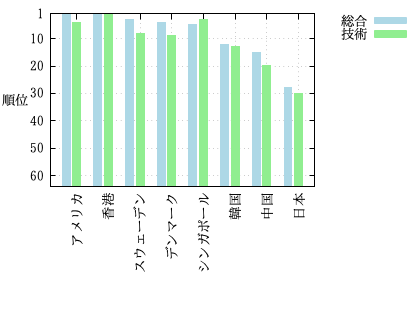
\includegraphics[width=0.7\linewidth]{グラフ.png}
    \caption{デジタル競争力ランキング}\label{fig:グラフ}
\end{figure}


% ーーー
% 節見出し(2)
\section{ブロードバンドの整備状況}
% 本文(2)
OECDによるブロードバンド回線の普及に関する調査\cite{oecd}によると,表\ref{tbl:加入率}に示すように,日本における
100人あたりのモバイルブロードバンドの加入者数は190.5で,第1位となっている.
2位はエストニアで,3位は米国と続く.
% 表の挿入
% \begin{tabular}
% \end{tabular}    
% による表の記述を 
% \begin{table}[htbp]
% \end{table}
% で囲み
% \caption{}
% で表のタイトルを入れる.
% \label{}
% を使って表番号が参照できるようにする
% また,
% \centering
% で表が中央に来るようにする
\begin{table}[htbp]
    \centering
    \caption{モバイルブロードバンドの加入者数(100人あたり)}
    \label{tbl:加入率}

    \begin{tabular}{|l|r|r|}\hline
        順位 & 国名 & 加入者数 \\
        \hline
        1位 & 日本 & 190.5 \\
        \hline
        2位 & エストニア & 179.9 \\
        \hline
        3位 & 米国 & 169.0 \\
        \hline
        4位 & フィンランド & 157.0 \\
        \hline
        5位 & デンマーク & 141.7 \\
        \hline
       6位 & ラトビア & 141.6 \\
        \hline 
       7位 & イスラエル & 139.9 \\
        \hline
       8位 & オランダ & 133.7 \\
        \hline
       9位 & ポーランド & 131.3 \\
        \hline
       10位 & スウェーデン & 127.2 \\
        \hline  
    \end{tabular}
\end{table}
% ーーー
% 見出し(3)
% 考察
%
% \begin{itemize}
% \end{itemize}
% を使って箇条書きで記述する
\section{考察}
-- 以上の調査結果について,自分が考えたことをここに書くこと --

\begin{itemize}
    \item 日本のブロードバンドの整備は世界トップ
    \item 日本のデジタル競争力は世界中位
    \item 技術革新の面で改善の余地がある
\end{itemize}
% ここに参考文献が入る
%

\bibliographystyle{junsrt}
\bibliography{exercise.bib}

\end{document}